\documentclass[12pt]{article}
\usepackage[utf8]{inputenc}

% Default fixed font does not support bold face
\DeclareFixedFont{\ttb}{T1}{txtt}{bx}{n}{12} % for bold
\DeclareFixedFont{\ttm}{T1}{txtt}{m}{n}{12}  % for normal

% Custom colors
\usepackage{color}
\definecolor{deepblue}{rgb}{0,0,0.5}
\definecolor{deepred}{rgb}{0.6,0,0}
\definecolor{deepgreen}{rgb}{0,0.5,0}
\setlength{\parskip}{2pt}%
\setlength{\parindent}{0pt}%
\usepackage{enumitem, amsmath, graphicx, wrapfig, float, nccmath, verbatim, fancyvrb, geometry, changepage, listings}
\usepackage[export]{adjustbox}
\newcommand\pythonstyle{\lstset{
		language=Python,
		basicstyle=\ttm,
		otherkeywords={self},             % Add keywords here
		keywordstyle=\ttb\color{deepblue},
		emph={MyClass,__init__},          % Custom highlighting
		emphstyle=\ttb\color{deepred},    % Custom highlighting style
		stringstyle=\color{deepgreen},
		frame=tb,                         % Any extra options here
		showstringspaces=false            % 
}}


% Python environment
\lstnewenvironment{python}[1][]
{
	\pythonstyle
	\lstset{#1}
}
{}

% Python for external files
\newcommand\pythonexternal[2][]{{
		\pythonstyle
		\lstinputlisting[#1]{#2}}}

% Python for inline
\newcommand\pythoninline[1]{{\pythonstyle\lstinline!#1!}}
\title{%
	ECE-471 Selected Topics in Machine Learning \\
	Prof. Curro \\
	Midterm Project}
\author{Evan Bubniak, Zhang Jinhan}
\begin{document}
\maketitle

\section{Summary}

The purpose of this project is to reproduce a subset of experimental results from the paper \textit{Understanding deep learning requires rethinking generalization} (Zhang et al. 2016), specifically Figure 1, which plots the average loss against the number of training steps for various types of example/label corruption. The experiment demonstrates that various kinds of label corruption do not prevent complete memorization of the training dataset, as long as the model is sufficiently large, and that the convergence of the model to 100\% accuracy is shifted by only a constant factor when data corruption is introduced.

Our results show strong agreement with Figure 1 for the first model specified, the minified InceptionV3, and strong divergence in all other models. The two models are displayed side-by-side. Crucially, we verify the key finding of the paper, which is the constant-factor difference in convergence time when introducing data and label corruption.

\begin{figure}[H]
	\centering
	\begin{minipage}{.5\textwidth}
		\centering
		\raisebox{-0.5\height}{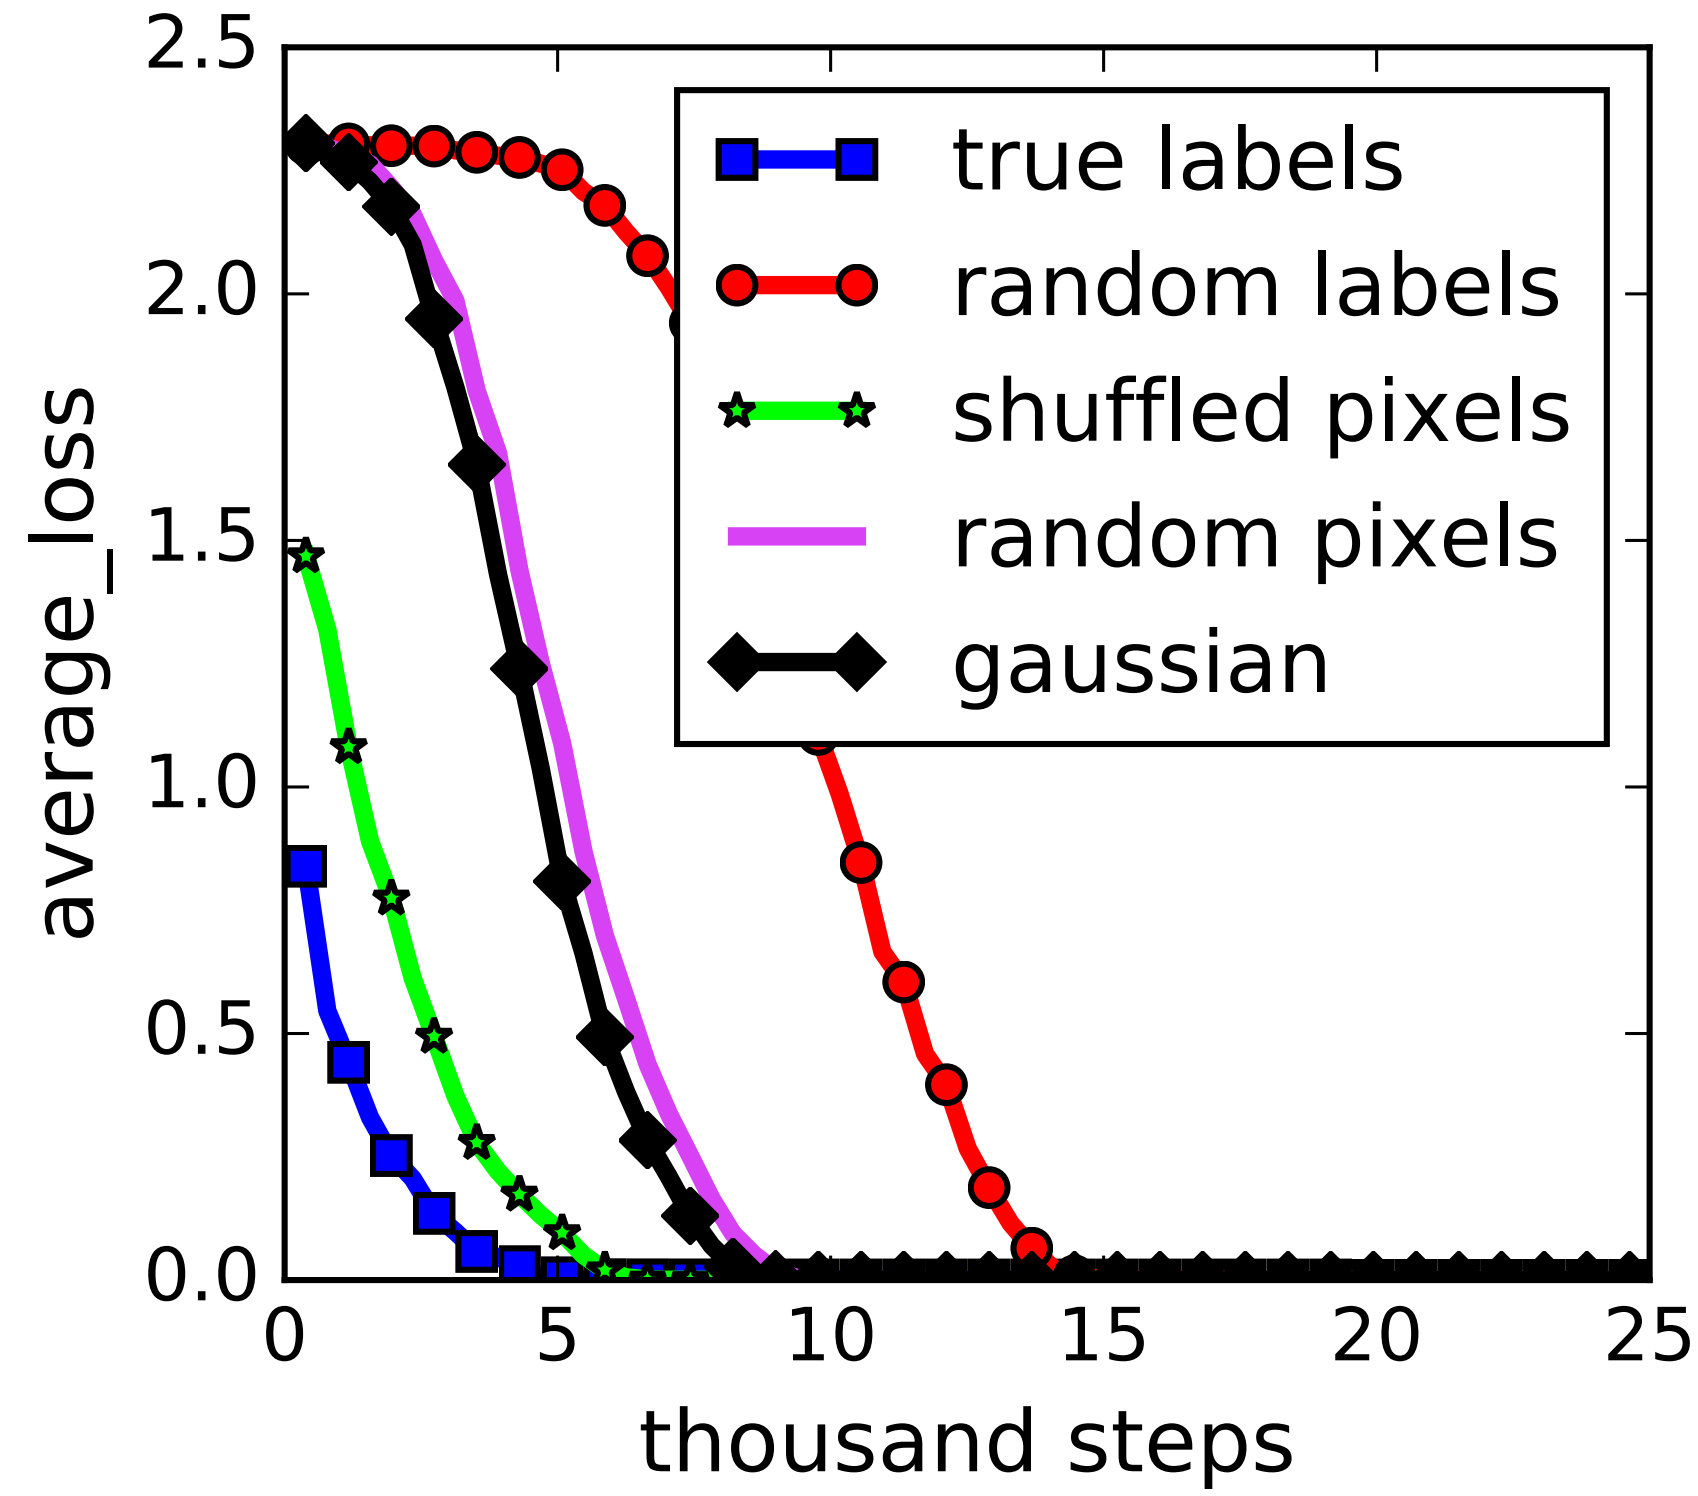
\includegraphics[width=0.8\linewidth]{fig.png}}
		\caption{A screenshot of the original figure as it appears in C. Zhang et al.}
		\raisebox{-0.5\height}{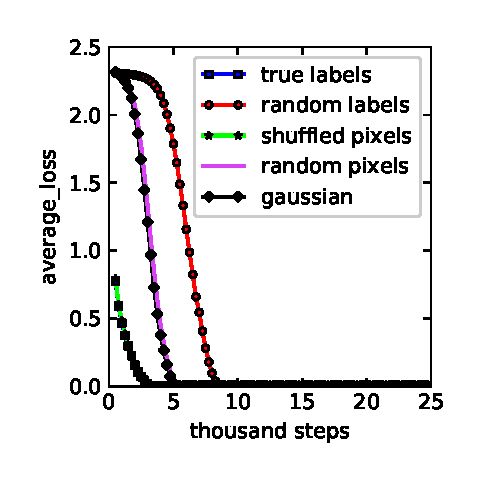
\includegraphics[width=0.875\linewidth]{C:/Users/evanb/Documents/deeplearning/midterm/output_2/MiniInceptionV3.eps}}
		\caption{A plot of the average losses for the minified InceptionV3 on the CIFAR-10 dataset, subject to various types of data corruption.}
	\end{minipage}
\end{figure}

\section{Experimental Setup}

We conducted many tests to reconstruct and verify the experimental setup. Specifically, we rebuilt each of the five models described in Table 1 of the original paper: two minified InceptionV3 models respectively with and without batch normalization, a minified AlexNet, and two multi-layer perceptions with 512 units and, respectively, one and three hideen layers. These models were built in Keras and the Python code defining them is provided in the appendix.

The experimental setup involved, in total, the training and analysis of 25 models, corresponding to five models each trained on five datasets. Training was performed on the KAHAN server and all plots were generated using Matplotlib.

The paper does not specify certain hyperparameters, specifically the number of epochs and batch size. This proved problematic as the interplay between these two variables affects the number of steps needed to converge. Furthermore, although five models are specified as part of the CIFAR-10 experimental set-up, it is not specified if only one model was used to generate Figure 1 in particular, or if multiple model results were averaged together.

As a result, some difference in the shape of the graph is likely due to hyperparameter tuning; specifically, we use a batch size of 200 and run on 100 epochs. Because $\frac{\text{\# training steps}}{\text{epoch}} = \frac{\text{\# samples}}{\text{batch size}}$, we choose the batch size and epochs such that, for 50,000 samples, we will have 25,000 training steps in total for each model run (thus spanning the width of the x-tick limits), and 250 steps per epoch (thus yielding a desirable width between data points), since data points are only logged at the end of each epoch in our Keras callback. We expect that a larger batch size should lead to a faster convergence for an otherwise fixed number of epochs.

\section{Things That Didn't Work}
\begin{figure}[H]
		\centering
		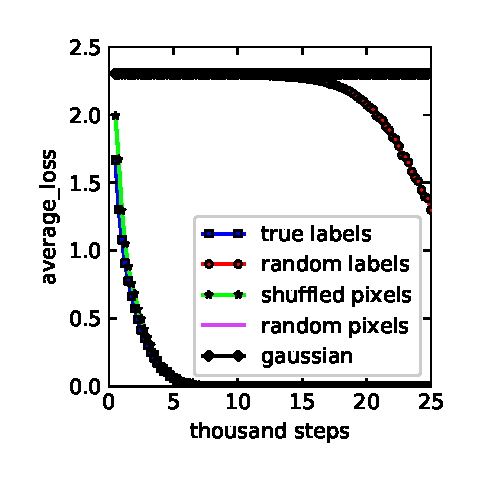
\includegraphics[width=0.45\textwidth]{C:/Users/evanb/Documents/deeplearning/midterm/output_2/MiniInceptionV3_without_BatchNorm.eps}
		\caption{Average losses for MiniInceptionV3 without BatchNorm.}
\end{figure}

\begin{figure}[H]
		\centering
		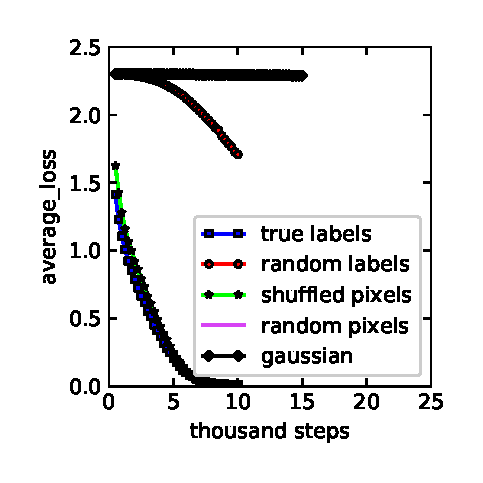
\includegraphics[width=0.45\textwidth]{C:/Users/evanb/Documents/deeplearning/midterm/output_2/AlexNet.eps}
		\caption{Average losses for AlexNet.}
\end{figure}

\begin{figure}[H]
		\centering
		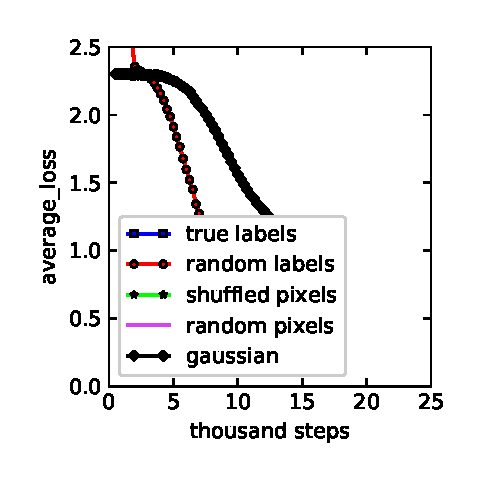
\includegraphics[width=0.45\textwidth]{C:/Users/evanb/Documents/deeplearning/midterm/output_2/MLP_1x512.eps}
		\caption{Average losses for MLP 1x512 without BatchNorm.}
\end{figure}

\begin{figure}[H]
		\centering
		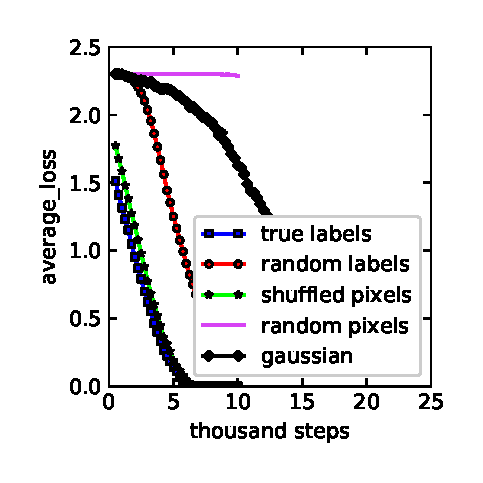
\includegraphics[width=0.45\textwidth]{C:/Users/evanb/Documents/deeplearning/midterm/output_2/MLP_3x512.eps}
		\caption{Average losses for MLP 3x512 without BatchNorm.}
\end{figure}

\begin{figure}[H]
	\centering
	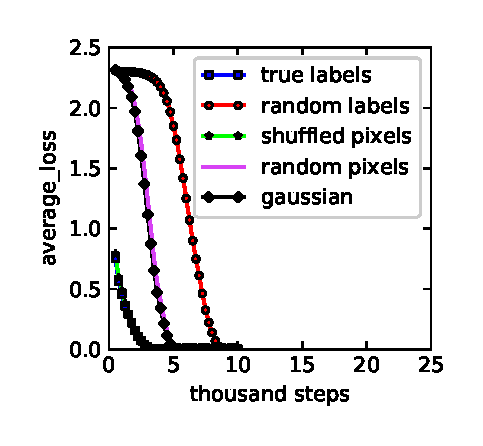
\includegraphics[width=0.45\textwidth]{C:/Users/evanb/Documents/deeplearning/midterm/output_2/output.eps}
	\caption{The average losses for each data type over all of the five models: MiniInceptionV3, MiniInceptionV3 w/o BatchNorm, AlexNet, the 1x512 MLP, and the 3x512 MLP.}
\end{figure}

\clearpage
\begin{adjustwidth}{-50pt}{0pt}

\section{Appendix}

For convenience of use, the \verb|main.py| and \verb|plot_results.py| scripts were augmented with command line argument parsing, giving strong user customization over which models to run on which data corruption, as well as being able to plot average losses for each data corruption type over several models.

\subsection{Main Loop}
\pythonexternal{C:/Users/evanb/Documents/deeplearning/midterm/main.py}

\subsection{Data Preprocessing}
\pythonexternal{C:/Users/evanb/Documents/deeplearning/midterm/utils/preprocess_data.py}

\subsection{Data Corruption}
\pythonexternal{C:/Users/evanb/Documents/deeplearning/midterm/utils/data_corruption.py}

\subsection{Model Definitions}
\pythonexternal{C:/Users/evanb/Documents/deeplearning/midterm/utils/Models.py}
\end{adjustwidth}

\subsection{Matplotlib configuation}
\pythonexternal{C:/Users/evanb/Documents/deeplearning/midterm/plot_results.py}

\end{document}